\documentclass{report}
\usepackage{hyperref}
\usepackage[margin=2.5cm]{geometry}
\usepackage{amsmath}
\usepackage{txfonts}
\usepackage{todonotes}
\usepackage{enumitem}
\usepackage{listings}
\usepackage{cleveref}

\usetikzlibrary{arrows.meta}

% https://tex.stackexchange.com/questions/229940/can-i-have-a-listing-with-fixed-column-code-and-full-flexible-comments
\makeatletter
\let\commentfullflexible\lst@column@fullflexible
\makeatother

% Use continuous footnote numbering so we can refer to them
% https://tex.stackexchange.com/questions/10448/continuous-footnote-numbering
\counterwithout{footnote}{chapter}

\lstset{
    language=haskell
  , basicstyle=\small\ttfamily
  , keywordstyle=\bfseries
  , commentstyle=\normalsize\rmfamily\itshape\commentfullflexible
  , columns=fixed
  , morekeywords={
        family
      , Type
      }
  }

\title{The IOHK Consensus and Storage Layer}
\author{Edsko de Vries \\ \href{mailto:edsko@well-typed.com}{edsko@well-typed.com}
   \and Duncan Coutts  \\ \href{mailto:duncan@well-typed.com}{duncan@well-typed.com} }

% TODO
%
% * Incorporate
%
%   - Previous blog posts
%   - Specifications currently stored as markdown files in the repo
%   - Any discussions in long comments in the code
%
% - choice of k: liveness versus safety
% - make sure we talk about the fact that the ledger can be linear

\newcommand{\duncan}{\todo{Duncan suitable section.}}

\begin{document}

\maketitle

\tableofcontents

\chapter{Introduction}

The IOHK Consensus and Storage layer, or \emph{the consensus layer} for short,
is a critical piece of infrastructure in the Cardano Node. It orchestrates
between the \emph{network layer} below it and the \emph{ledger layer} above it.

The network layer is a highly concurrent piece of software that deals with
low-level concerns; its main responsiblity is to transmit data efficiently
across the network. Although it primarily transmits blocks and block headers, it
does not interpret them and does not need to know much about them. In the few
cases where it \emph{does} need to make some block-specific decisions, it
calls back into the consensus layer to do so.

The ledger layer by contrast exclusively deals with high-level concerns. It is
entirely stateless: its main responsibility is to define a single pure
function describing how the ledger state is transformed by blocks (verifying
that blocks are valid in the process). It is only concerned with linear history;
it is not aware of the presence of multiple competing chains or the roll backs
required when switching from one chain to another.

The consensus layer mediates between these two layers. It includes a
bespoke storage layer that provides efficient access to the current ledger state
as well as both (recent) \emph{past} ledger states (required in order to be able
to validate and switch to competing chains) as well as (views on near)
\emph{future} ledger states (required to be able to validate block headers
without access to the corresponding block bodies). The storage layer also
provides direct access to the blocks on the blockchain itself,  so that they can
be efficiently streamed to clients (via the network layer). When there are
competing chains, the consensus layer decides which chain is preferable and
should be adopted, and it decides when to \emph{contribute} to the chain
(produce new blocks). All ``executive decisions'' about the chain are made in
and by the consensus layer.

Lastly, as well we see, the consensus layer is highly abstract and places a
strong emphasis on compositionality, making it useable with many different
consensus algorithms and ledgers. Importantly, compositionality enables the
\emph{hard fork combinator} to combine multiple ledgers and regard them as a
single block chain.

The goal of this document is to outline the design goals for the consensus
layer, how we achieved them, and where there is still scope for improvement. We
will both describe \emph{what} the consensus layer is, and \emph{why} it is the
way it is. Throughout will also discuss what \emph{didn't} work, approaches we
considered but rejected, or indeed adopted but later abandoned; discussing these
dead ends is sometimes at least as informative as discussing the solution that
did work.

We will consider some of the trade-offs we have had to make, how they
affected the development, and discuss which of these trade-offs should perhaps
be reconsidered. We will also take a look at how the design can scale to
facilitate future requirements, and which requirements will be more problematic
and require more large-scale refactoring.

The target audience for this document is primarily developers working on the
consensus layer. It may also be of more broader interest to people generally
interested in the Cardano block chain, although we will assume that the
reader has a technical background.

\chapter{Overview}

\section{Components}

\subsection{Consensus protocols}
\label{overview:consensus}

The consensus protocol has two primary responsibilities:
\label{consensus-responsibilities}

\begin{description}
\item[Chain selection] Competing chains arise when two or more nodes extend the
chain with different blocks. This can happen when nodes are not aware of each
other's blocks due to temporarily network delays or partitioning, but depending
on the particular choice of consensus algorithm it can also happen in the normal
course of events. When it happens, it is the responsibility of the consensus
protocol to choose between these competing chains.

\item[Leadership check] In proof-of-work blockchains any node can produce a
block at any time, provided that they have sufficient hashing power. By
contrast, in proof-of-stake time is divided into \emph{slots}, and each slot has
a number of designated \emph{slot leaders} who can produce blocks in that slot.
It is the responsibility of the consensus protocol to decide on this mapping
from slots to slot leaders.
\end{description}

The consensus protocol will also need to maintain its own state; we will discuss
state management in more detail in \cref{state}.

\subsection{Ledger}
\label{overview:ledger}

The role of the ledger is to define what is stored \emph{on} the blockchain.
From the perspective of the consensus layer, the ledger has three primary
responsibilities:

\begin{description}
\item[Applying blocks] The most obvious and most important responsibility of
the ledger is to define how the ledger state changes in response to new blocks,
validating blocks at it goes and rejecting invalid blocks.

\item[Ticking time] Some parts of the ledger state change due to the passage of
time only. For example, blocks might \emph{schedule} some changes to be applied
later, and then when the relevant slot arrives those changes should be applied,
independent from any blocks.

\item[Forecasting] Some consensus protocols require limited information from the
ledger. In Praos, for example, a node's probability of being a slot leader is
proportional to its stake, but the stake distribution is something that the
ledger keeps track of. We refer to this as a \emph{view} on the ledger, and we
require not just that the ledger can give us a view on the \emph{current} ledger
state, but also \emph{predict} what that view will be for slots in the near
future. We will discuss the motivation for this requirement in
\cref{header-body}.
\end{description}

The primary reason for separating out ``ticking'' from applying blocks is that
the consensus layer is responsible to the leadership check
(\cref{consensus-responsibilities}), and when we need to decide if we should be
producing a block in a particular slot, we need to know the ledger state at that
slot (even though we don't have a block for that slot \emph{yet}). It is also
required in the mempool; see \cref{mempool}.

\section{Design Goals}

\subsection{Multiple consensus protocols}
\label{multiple-consensus-protocols}

From the beginning it was clear that we would need support for multiple
consensus algorithms: the Byron era uses a consensus algorithm called BFT
(\cref{bft}) and the Shelley era uses a consensus algorithm called
Praos (\cref{praos}). Moreover, the Cardano blockchain is a \emph{hybrid}
chain where the prefix of the chain runs Byron (and thus uses BFT), and then
continues with Shelley (and thus uses Praos); we will come back to the topic
of composing protocols when we discuss the hard fork combinator (\cref{hfc}).
It is therefore important that the consensus layer abstracts over a choice
of consensus protocol.

\subsection{Support for multiple ledgers}
\label{multiple-ledgers}

For much the same reason that we must support multiple consensus protocols, we
also have to support multiple ledgers. Indeed, we expect more changes in ledger
than in consensus protocol; currently the Cardano block chain starts with a
Byron ledger and then transitions to a Shelley ledger, but further changes to
the ledger have already been planned (some intermediate ledgers currently
code-named Allegra and Mary, as well as larger updates to Goguen, Basho and
Voltaire). All of the ledgers (Shelley up to including Voltaire)
use the Praos consensus algorithm (potentially extended with the genesis chain
selection rule, see \cref{future:genesis}).

\subsection{Decouple consensus protocol from ledger}
\label{decouple-consensus-ledger}

As we saw above (\cref{multiple-ledgers}), we have multiple ledgers that all
use the same consensus protocol. We therefore should be able to define the
consensus protocol \emph{independent} from a particular choice of ledger,
merely defining what the consensus protocol expects from the ledger
(we will see what this interface looks like in \cref{ledger}).

\subsection{Testability}
\label{testability}

The consensus layer is a critical component of the Cardano Node, the software
that runs the Cardano blockchain. Since the blockchain is used to run the Ada
cryptocurrency, it is of the utmost importance that this node is reliable;
network downtime or, worse, corruption of the blockchain, cannot be tolerated.
As such the consensus layer is subject to much stricter correctness criteria
than most software, and must be tested thoroughly. To make this possible, we
have to design for testability.

\begin{itemize}
\item We must be able to simulate various kinds of failures (disk
failures, network failures, etc.) and verify that the system can recover.
\item We must be able to run \emph{lots} of tests which means that tests need to
be cheap. This in turn will require for example the possibility to swap the
cryptographic algorithms for much faster ``mock'' crypto algorithms.
\item We must be able to test how the system behaves under certain
expected-but-rare circumstances. For example, under the Praos consensus
protocol it can happen that a particular slot has multiple leaders. We should be
able to test what happens when this happens repeatedly, but the leader selection
is a probabilistic process; it would be difficult to set up test scenarios to
test for this specifically, and even more difficult to set things up so that
those scenarios as \emph{shrinkable} (leading to minimal test cases). We must
therefore be able to ``override'' the behaviour of the consensus protocol (or
indeed the ledger) at specific points.
\item We must be able test components individually (rather than just the system
as a whole), so that if a test fails, it is much easier to see where something
went wrong.
\end{itemize}

\subsection{Adaptability and Maintainability}
\label{adaptability}

The Cardano Node began its life as an ambitious replacement of the existing
prototype implementation of the Cardano blockchain, which had been developed
by Serokell. At the time, the Shelley ledger was no more than an idea, and
the Praos consensus protocol existed only as a research paper. Moreover, since
the redesign would be unable to reuse any parts of the prototype, even the
Byron ledger did not yet exist when the consensus layer was started.
It was therefore important from the get-go that the consensus layer was not
written for a specific ledger, but rather abstract over a choice of ledger
and define precisely what the responsibilities of that ledger were.

This abstraction over both the consensus algorithm and the ledger is important
for other reasons, too. As we've mentioned, although initially developed to
support the Byron ledger and the (P)BFT consensus algorithm, the goal was to
move to Shelley/Praos as quickly as possible. Moreover, additional ledgers had
already been planned (Goguen, Basho and Voltaire), and research on consensus
protocols was (and still is) ongoing. It was therefore important that the
consensus layer could easily be adapted.

Admittedly, adaptability does not \emph{necessarily} require abstraction. We
could have built the consensus layer against the Byron ledger initially
(although we might have had to wait for it to be partially completed at least),
and then generalize as we went. There are however a number of downsides to this
approach.

\begin{itemize}
\item When working with a concrete interface, it is difficult to avoid certain
assumptions creeping in that may hold for this ledger but will not hold for
other ledgers necessarily. When such assumptions go unnoticed, it can be costly
to adjust later. (For one example of such an assumption that nonetheless
\emph{did} go unnottced, despite best efforts, and took a lot of work to
resolve, see \cref{removing-known-slot-assumption} on removing the assumption
that we can always convert between wallclock time and slot number.)

\item IOHK is involved in the development of blockchains other that Cardano too,
and the hope is that the consensus layer can be used in those projects as well.

\item Perhaps most importantly, if the consensus layer only supports a single,
concrete ledger, it would be impossible to \emph{test} the consensus layer with
any ledgers other than that concrete ledger. But this means that all consensus
tests need to deal with all the complexities of the real ledger. By constrast,
by staying abstract, we can run a lot of consensus tests with mock ledgers that
are easier to set up, easier to reason about, more easily instrumented and more
amenable to artificially creating rare circumstances (see \cref{testability}).
\end{itemize}

Of course, abstraction is also just good engineering practice. Programming
against an abstract interface means we are clear about our assumptions,
decreases dependence between components, and makes it easier to understand and
work with individual components without having to necessarily understand the
entire system as a whole.

\subsection{Composability}
\label{composability}

The consensus layer is a complex piece of software;  at the time we are writing
this techical report, it consists of roughly 100,000 lines of code. It is
therefore important that we split it into into small components that can be
understood and modified independently from the rest of the system. Abstraction,
discussed in \cref{adaptability}, is one technique to do that, but by no means
the only. One other technique that we make heavy use of is composability. We
will list two examples here:

\begin{itemize}
\item As discussed in \cref{multiple-consensus-protocols} and
\cref{multiple-ledgers}, the Cardano blockchain has a prefix that runs the BFT
consensus protocol and the Byron ledger, and then continues with the Praos
consensus protocol and the Shelley ledger. We do not however define a consensus
protocol that is the combination of Byron and Praos, nor a ledger that is the
combination of Byron and Shelley. Instead, the \emph{hard fork combinator}
(\cref{hfc}) makes it possible to \emph{compose} consensus protocols and
ledgers: construct the hybrid consensus protocol from an implementation of BFT
and an implementation of Praos, and similarly for the ledger.

\item We mentioned in \cref{testability} that it is important that we can
test the behaviour of the consensus layer under rare-but-possible circumstances,
and that it is therefore important that we can override the behaviour of the
consensus algorithm in tests. We do not accomplish this however by adding
special hooks to the Praos consensus algorithm (or any other); instead we define
another combinator that takes the implementation of a consensus algorithm and
\emph{adds} additional hooks for the sake of the testing infrastructure. This
means that the implementation of Praos does not have to be aware of testing
constraints, and the combinator that adds these testing hooks does not need to
be aware of the details of how Praos is implemented.
\end{itemize}

\subsection{Predictable Performance}

Make sure node operators do not set up nodes for "normal circumstances" only
for the network to go down when something infrequent (but expected) occurs.
(This is not about malicious behaviour, that's the next section).

\duncan

\subsection{Protection against DoS attacks}

Brief introduction to asymptotic attacker/defender costs. (This is just an
overview, we come back to these topics in more detail later.)

\duncan

\chapter{Non-functional requirements}

This whole chapter is Duncan-suitable :)
\duncan

\section{Network layer}

This report is not intended as a comprehensive discussion of the network layer;
see \cite{network-spec} instead. However, in order to understand
some of the design decisions in the consensus layer we need to understand some
of the requirements imposed on it by the network layer.

TODOs:

\begin{itemize}
\item Highlight relevant aspects of the design of the network layer
\item Discuss requirements this imposes on the consensus layer
Primary example: Forecasting.
\item How do we keep the overlap between network and consensus as small
as possible? Network protocols do not involve consensus protocols
(chain sync client is not dependent on chain selection). Chain sync
client + "pre chain selection" + block download logic keeps things isolated.
\item Why do we even want to validate headers ahead of time? (Thread model etc.)
(Section for Duncan?).
Section with a sketch on an analysis of the amortized cost for attackers versus
our own costs to defend against it ("budget for work" that grows and shrinks
as you interact with a node).
\end{itemize}

\subsection{Header/Body Split (aka: Header submission)}
\label{header-body}

Discuss the chain fragments that we store per upstream node.
Discuss why we want to validate headers here -- without a full ledger state
(necessarily so, since no block bodies -- can't update ledger state)
(\cref{ledger:forecasting} contains a discussion of this from the pov of
the ledger).
Discuss why it's useful if the chain sync client can race ahead  for
\emph{performance} (why it's required for chain selection is the discussed in
\cref{forecast:ledgerview}).

\subsection{Block submission}
\label{network:blocksubmission}

\subsection{Transaction submission}
\label{network:txsubmission}

\section{Security "cost" concerns}

TODO: Look through the code and git history to find instances of where we
one way but not the other because it would give an attacker an easy way to
make it do lots of work (where were many such instances).

Fragile. Future work: how might be make this less brittle?
Or indeed, how might we test this?

Counter-examples (things we don't want to do)

\begin{itemize}
\item Parallel validation of an entire epoch of data (say, crypto only).
You might do a lot of work before realizing that that work was not needed because
of an invalid block in the middle.
\end{itemize}

Future work: opportunities for parallelism that we don't yet exploit
(important example: script evaluation in Goguen).

\section{Hard time constraints}

Must produce a block on time, get it to the next slot leader

Bad counter-example: reward calculation in the Shelley ledger bad
(give examples of why).

\section{Predictable resource requirements}

make best == worst

(not \emph{just} a security concern: a concern even if every node honest)

\chapter{Consensus Protocol}

% TODO: what kind of variation does this design support?
% (counter-example: genesis rule)

% TODO: Describe API
%
% TODO: State invariants
%
% TODO: Discuss relationship to the Ouroboros papers. Where are the various parts
% of the paper implemented? How do additional design constraints change this?
% (e.g. header/body split)

\section{Fundamental parameters}

\subsection{The security parameter $k$}
\label{param:k}

\section{Chain selection}
\label{chain-selection}

\subsection{Overview}
\label{chain-selection:overview}

Chain selection is the process of choosing between multiple competing chains,
and is one of the most important responsibilities of a consensus protocol. When
choosing between two chains, in theory any part of those chains could be
relevant; indeed, in the research papers chain selection is described as a
comparison of two entire chains (\cref{bft-paper,praos-paper}). In practice that
is not realistic: the node has to do chain selection frequently, and scanning
millions of blocks each time to make the comparison is of course out of the
question.

The consensus layer keeps the last $k$ blocks as a \emph{chain fragment} in
memory (\cref{in-memory}); the rest of the chain is stored on disk. Similarly,
we keep a chain fragment of \emph{headers} in memory for every (upstream) node
whose chain we are following and whose blocks we may wish to adopt
(\cref{header-body}). Before the introduction of the hard fork combinator chain
selection used to be given these fragments to compare; as we will discuss in
\cref{simplifying-chain-selection}, however, this does not scale so well to
hybrid chains.

It turns out, however, that it suffices to look only at the block at the very
tip of the chain\footnote{This does give rise to the question of what to do when
there \emph{is} no block on the chain, and indeed to the---signifcantly more
subtle---question of what to do when there is no block on one of the
\emph{fragments}. We will come back to this in detail in
\cref{simplifying-chain-selection}.}, at least for the class of consensus
algorithms we need to support. The exact information we need about that tip
varies from one protocol to the other, but at least for the Ouroboros family of
consensus protocols the essence is always the same: we prefer longer chains over
shorter ones (justifying \emph{why} this is the right choice is the domain  of
cryptographic research and well outside the scope of this report). In the
simplest case, the length of the chain is \emph{all} that matters, and hence the
only thing we need to know about the blocks at the tips of the chains is their
block numbers.\footnote{This is not \emph{entirely} true, due to the presence of
EBBs; see \cref{ebb-chain-selection}.}

\subsection{Interface}
\label{chain-selection:interface}

We model chain selection as its own class\footnote{Here and elsewhere we elide
superclass constraints that are not relevant to the discussion.}, separate from
the full consensus algorithm (\cref{class:ConsensusProtocol}); this will allow
us to more easily override this aspect of a consensus protocol when needed; see
\cref{consensus:override-leader-schedule}.

\begin{lstlisting}
class (..) => ChainSelection p where
\end{lstlisting}

The type variable $p$ is a type-level tag describing a particular consensus
protocol; if Haskell had open kinds, we could say \lstinline!(p :: ConsensusProtocol)!. Like most other things, chain selection may require
some static configuration data, although most chain selection algorithms do
not:\footnote{Explicitly modelling such a required context could be avoided if
we used explicit records instead of type classes; we will discuss this point in
more detail in \cref{classes-vs-records}.}

\begin{lstlisting}
type family ChainSelConfig p :: Type
type ChainSelConfig p = ()
\end{lstlisting}

As mentioned in \cref{chain-selection:overview}, chain selection will only look
at the headers at the tip of the ledger. Since we are defining consensus
protocols independent from a concrete choice of ledger, however
(\cref{decouple-consensus-ledger}), we cannot use a concrete block or header
type. Instead, we merely say that the chain selection requires \emph{some} view
on headers that it needs to make its decisions:

\begin{lstlisting}
type family SelectView p :: Type
type SelectView p = BlockNo
\end{lstlisting}

The default is \lstinline!BlockNo! because as we have seen this is all that is
required for the most important chain selection rule, simply preferring longer
chains over shorter ones. It is the responsibility of the glue code that
connects a specific choice of ledger to a consensus protocol to define the
projection from a concrete block type to this \lstinline!SelectView!
(\ref{BlockSupportsProtocol}).

Chain selection itself then is modelled as a pair of functions: one that checks
if we prefer a \emph{candidate} chain (that is, chains other than our own) to
our own chain, and one that compares two candidate chains:
\todo{Both of these functions have preconditions. We should discuss those and
where we rely on them.}

\begin{lstlisting}
preferCandidate   :: proxy          p
                  -> ChainSelConfig p
                  -> SelectView     p      -- ^ Tip of our chain
                  -> SelectView     p      -- ^ Tip of the candidate
                  -> Bool

compareCandidates :: proxy          p
                  -> ChainSelConfig p
                  -> SelectView     p
                  -> SelectView     p
                  -> Ordering
\end{lstlisting}

We separate these out because the Ouroboros consensus protocols treat these
cases differently: candidate chains of equal length are equally preferable
(we could choose either one), but a candidate chain is only preferred over our
current chain if it is \emph{strictly} longer. These functions have default
implementation that use the default \lstinline!SelectView! and implement
the longest chain rule:

\begin{lstlisting}
preferCandidate   _ _ ours cand = compare ours cand == LT
compareCandidates _ _           = compare
\end{lstlisting}

\section{Full protocol}
\label{class:ConsensusProtocol}

The main class modelling the consensus protocol has chain selection as a
superclass constraint:

\begin{lstlisting}
class (ChainSelection p, ..) => ConsensusProtocol p where
\end{lstlisting}

As for leader selection (and most of our other key abstractions), the consensus
protocol may need its own configuration; the remainder of the class itself is
split into two parts: the first part deals with updating the \emph{state} of the
consensus protocol, and the second deals with leader selection. We will discuss
these separately.

\subsection{Configuration}
\label{class:ConsensusProtocol:config}

Each consensus protocol defines its own type of required static
configuration:\footnote{This is defined as a data family rather than a type
family: since all functions in the class take the configuration as an argument,
it can serve as a hint to the type checker about which protocol we're interested
in, avoiding the need for an explicit proxy. We did not do that for chain
selection because there it was more useful to be able to specify a default (most
chain selection algorithms don't require configuration), which is not possible
with a data family.}

\begin{lstlisting}
data family ConsensusConfig p :: Type
\end{lstlisting}

Since chain selection is part of the consensus protocol, the chain selection
config should be a subset of the full protocol config:

\begin{lstlisting}
chainSelConfig :: ConsensusConfig p -> ChainSelConfig p
\end{lstlisting}

The rest of the consensus layer does not really do much with this configuration,
except make it available where required; however, we do require that whatever
the configuration is, we can extract $k$ from it:

\begin{lstlisting}
protocolSecurityParam :: ConsensusConfig p -> SecurityParam
\end{lstlisting}

For example, this is used by the chain database to determine when blocks can be
moved from the volatile DB to the immutable DB
(\cref{immutable-volatile-split}).

\subsection{Ledger view}
\label{class:ConsensusProtocol:ledgerview}

We mentioned in \cref{overview:ledger} that some consensus protocols may require
limit information from the ledger; for instance, the Praos consensus protocol
needs access to the stake distribution for the leadership check. In the
\lstinline!ConsensusProtocol! abstraction, this is modelled as a \emph{view}
on the ledger state

\begin{lstlisting}
type family LedgerView p :: Type
\end{lstlisting}

The ledger view will be required in only one function: when we ``tick'' the
state of the consensus protocol. We will discuss this state management in more
detail next.

\subsection{Protocol state management}
\label{class:ConsensusProtocol:state}

Each consensus protocol has its own type chain dependent state\footnote{We are
referring to this as the ``chain dependent state'' to emphasize that this is
state that evolves with the chain, and indeed is subject to rollback when we
switch to alternatives forks. This distinguishes it from chain
\emph{independent} state such as evolving private keys, which are updated
independently from blocks and are not subject to rollback.}

\begin{lstlisting}
type family ChainDepState p :: Type
\end{lstlisting}

The state must be updated with each block that comes in, but just like for
chain selection, we don't work with a concrete block type but instead define a
\emph{view} on blocks that is used to update the consensus state:

\begin{lstlisting}
type family ValidateView p :: Type
\end{lstlisting}

We're referring to this as the \lstinline!ValidateView! because updating the
consensus state also serves as \emph{validation} of (that part of) the block;
consequently, validation can also \emph{fail}, with protocol specific error
messages:

\begin{lstlisting}
type family ValidationErr p :: Type
\end{lstlisting}

Updating the chain dep state now comes as a pair of functions. As for the ledger
(\cref{overview:ledger}), we first \emph{tick} the protocol state to the
appropriate slot, passing the already ticked ledger view as an
argument:\footnote{Throughout the consensus layer, the result of ticking is
distinguished from the unticked value at the type level. This allows to store
additional (or indeed, less) information in the ticked ledger state, but also
clarifies ordering. For example, it is clear in \lstinline!tickChainDepState!
that the ledger view we pass as an argument is already ticked, as opposed to the
\emph{old} ledger view.}

\begin{lstlisting}
tickChainDepState ::
     ConsensusConfig p
  -> Ticked (LedgerView p)
  -> SlotNo
  -> ChainDepState p
  -> Ticked (ChainDepState p)
\end{lstlisting}

As an example, the Praos consensus protocol (\cref{praos}) derives its
randomness from the  chain itself. It does that by maintaining a set of random
numbers called \emph{nonces}, which are used as seeds to pseudo-random number
generators. Every so often the current nonce is swapped out for a new one; this
does not depend on the specific block, but merely on a certain slot number being
reached, and hence is an example of something that the ticking function should
do.

The (validation view on) a block can then be applied to the already ticked
protocol state:

\begin{lstlisting}
updateChainDepState ::
     ConsensusConfig       p
  -> ValidateView          p
  -> SlotNo
  -> Ticked (ChainDepState p)
  -> Except (ValidationErr p) (ChainDepState p)
\end{lstlisting}

Finally, there is a variant of this function that can we used to \emph{reapply}
a known-to-be-valid block, potentially skipping expensive cryptographic checks,
merely computing what the new state is:

\begin{lstlisting}
reupdateChainDepState ::
     ConsensusConfig       p
  -> ValidateView          p
  -> SlotNo
  -> Ticked (ChainDepState p)
  -> ChainDepState         p
\end{lstlisting}

Re-applying previously-validated blocks happens when we are replaying blocks
from the immutable database when initializing the in-memory ledger state (\cref{state:initialization}). It is also useful during chain selection (\cref{state:chainselection}): depending on the consensus protocol, we may end
up switching relatively frequently between short-lived forks; when this happens,
skipping expensive checks can improve the performance of the node.
\todo{How does this relate to the best case == worst case thing? Or to the
asymptotic attacker/defender costs?}

\subsection{Leader selection}
\label{class:ConsensusProtocol:leaderselection}

The final responsibility of the consensus protocol is leader selection. First,
it is entirely possible for nodes to track the blockchain without ever producing
any blocks themselves; indeed, this will be the case for the majority of
nodes\footnote{Most ``normal'' users will not produce blocks themselves, but
instead delegate their stake to stakepools who produce blocks on their behalf.}
In order for a node to be able to lead at all, it may need access to keys and
other configuration data; the exact nature of what is required is different
from protocol to protocol, and so we model this as a type family

\begin{lstlisting}
type family CanBeLeader p :: Type
\end{lstlisting}

A value of \lstinline!CanBeLeader! merely indicates that the node has the
required configuration to lead at all. It does \emph{not} necessarily mean that
the node has the right to lead in any particular slot; \emph{this} is indicated
by a value of type \lstinline!IsLeader!:

\begin{lstlisting}
type family IsLeader p :: Type
\end{lstlisting}

In simple cases \lstinline!IsLeader! can just be a boolean value (``yes, you are
a leader now'' or ``no, you are not leading in this slot'') but for more
sophisticated consensus protocols such as Praos this will be a cryptographic
proof that the node indeed has the right to lead in this slot. Checking whether
a that \emph{can} lead \emph{should} lead in a given slot is the responsibility
of the final function in this class:

\begin{lstlisting}
checkIsLeader ::
     ConsensusConfig       p
  -> CanBeLeader           p
  -> SlotNo
  -> Ticked (ChainDepState p)
  -> Maybe (IsLeader       p)
\end{lstlisting}

\section{Connecting a block to a protocol}
\label{BlockSupportsProtocol}

Although a single consensus protocol might be used with many blocks, any given
block is designed for a \emph{single} consensus protocol. The following type
family witnesses this relation:
%
\begin{lstlisting}
type family BlockProtocol blk :: Type
\end{lstlisting}
%
Of course, for the block to be useable with that consensus protocol, we need
functions that construct the \lstinline!SelectView!
(\cref{chain-selection:interface}) and \lstinline!ValidateView!
(\cref{class:ConsensusProtocol:state}) projects from that block:
%
\begin{lstlisting}
class (..) => BlockSupportsProtocol blk where
  validateView ::
       BlockConfig blk
    -> Header blk -> ValidateView (BlockProtocol blk)

  selectView ::
       BlockConfig blk
    -> Header blk -> SelectView (BlockProtocol blk)
\end{lstlisting}
%%
The \lstinline!BlockConfig! is the static configuration required to work with
blocks of this type; it's just another data family:
%
\begin{lstlisting}
data family BlockConfig blk :: Type
\end{lstlisting}

\section{Permissive BFT}
\label{bft}

Defined in \cite{byron-chain-spec}
Not to be confused with ``Practical BFT'' \cite{10.1145/571637.571640}

\subsection{Background}
\label{bft:background}

\duncan
Discuss \emph{why} we started with Permissive BFT (backwards compatible with
Ouroboros Classic).

\subsection{Implementation}

\subsection{Relation to the paper}
\label{bft-paper}

Permissive BFT is a variation on Ouroboros BFT, defined in
\cite{cryptoeprint:2018:1049}. We have included the main protocol description
from that paper as \cref{figure:bft} in this document; the only difference is
that we've added a few additional labels so we can refer to specific parts of
the protocol description below.

It will be immediately obvious from \cref{figure:bft} that this description
covers significantly more than what we consider to be part of the consensus
protocol proper here. We will discuss the various parts of the BFT protocol
description below.

\begin{description}
  \item[Clock update and network delivery] The BFT specification requires that
  ``with each advance of the clock (..) a collection of transactions and
  blockchains are pushed to the server''. We consider neither block submission
  nor transaction submission to be within the scope of the consensus algorithm;
  see \cref{network:blocksubmission,network:txsubmission} instead, respectively.

  \item[Mempool update] (\cref{bft:mempool}). The design of the mempool is the
  subject of \cref{mempool}. Here we only briefly comment on how it relates to
  what the BFT specification assumes:
%
  \begin{itemize}
    \item \textit{Consistency} (\cref{bft:mempool:consistency}). Our mempool
    does indeed ensure consistency. In fact, we require something strictly
    stronger; see \cref{mempool:consistency} for details.
    \item \textit{Time-to-live (TTL)} (\cref{bft:mempool:ttl}). The BFT
    specification requires that transactions stay in the mempool for a maximum
    of $u$ rounds, for some configurable $u$. Our current mempool does not have
    explicit support for a TTL parameter. The Shelley ledger will have support
    for TTL starting with the ``Allegra'' era, so that transactions are only
    valid within a certain slot window; this is part of the normal ledger rules
    however and requires no explicit support from the consensus layer. That's
    not to say that explicit support would not be useful; see \cref{future:ttl}
    in the chapter on future work.
    \item \textit{Receipts} (\cref{bft:mempool:receipts}). We do not offer any
    kind of receipts for inclusion in the mempool. Clients such as wallets must
    monitor the chain instead (see also \cite{wallet-spec}). The BFT
    specification marks this as optional so this is not a deviation.
  \end{itemize}
%
  \item[Blockchain update] (\cref{bft:update}). The BFT specification requires
  that the node prefers any valid chain over its own, as long as its strictly
  longer. \emph{We do not satisfy this requirement.} The chain selection rule
  for Permissive BFT is indeed the longest chain rule, \emph{but} consensus
  imposes a global maximum rollback (the security parameter $k$;
  \cref{param:k}). In other words, nodes \emph{will} prefer longer chains over
  its own, \emph{provided} that the intersection between that chain and the
  nodes own chain is no more than $k$ blocks away from the node's tip.
  \todo{Justify this maximum rollback?}

  Moreover, our definition of validity is also different. We do require that
  hashes line up (\cref{bft:update:hash}), although we do not consider this part
  of the responsibility of the consensus protocol, but instead require this
  independent of the choice of consensus protocol when updating the header state
  (\cref{state:header}). We do of course also require that the transactions in
  the block are valid (\cref{bft:update:body}), but this is the responsibility
  of the ledger layer instead (\cref{ledger}); the consensus protocol should be
  independent from what's stored in the block body.

  Permissive BFT is however different from BFT \emph{by design} in the
  signatures we require.\footnote{\label{footnote:singlesignature}There is
  another minor deviation from the specification: we don't require an explicit
  signature on the block body. Instead, we have a single signature over the
  header, and the header includes a \emph{hash} of the body.} BFT requires that
  each block is signed strictly according to the round robin schedule
  (\cref{bft:update:signatures}); the whole point of \emph{permissive} BFT is
  that we relax this requirement and merely require that blocks are signed by
  \emph{any} of the known core nodes.

  Permissive BFT is however not \emph{strictly} more permissive than BFT:
  although blocks do not need to be signed according to the round robin
  schedule, there is a limit on the number of signatures by any given node in a
  given window of blocks. When a node exceeds that threshold, its block is
  rejected as invalid. Currently that threshold is set to 0.22 \cite[Appendix A,
  Calculating the $t$ parameter]{byron-chain-spec}, which was considered to be
  the smallest value that would be sufficiently unlikely to consider a chain
  generated by Ouroboros Classic as invalid (\cref{bft:background}) and yet give
  as little leeway to a malicious node as possible. This has an unfortunate side
  effect, however. BFT can always recover from network partitions \cite[Section
  1, Introduction]{cryptoeprint:2018:1049}, but this is not true for PBFT: in a
  setting with 7 core nodes (the same setting as considered in the PBFT
  specification), a 4:3 network partition would quickly lead to \emph{both}
  partitions being unable to produce more blocks; after all, the nodes in the
  partition of 4 nodes would each sign 1/4th of the blocks, and the nodes in the
  partition of 3 nodes would each sign 1/3rd. Both partitions would therefore
  quickly stop producing blocks. Picking 0.25 for the threshold instead of 0.22
  would alleviate this problem, and would still be conform the PBFT
  specification, which says that the value must be in the closed interval
  $[\frac{1}{5}, \frac{1}{4}]$. Since PBFT is however no longer required (the
  Byron era is past and fresh deployments would not need Permissive BFT but
  could use regular BFT), it's probably not worth reconsidering this, although
  it \emph{is} relevant for the consensus tests (\cref{testing:dire}).
%
  \item[Blockchain extension] (\cref{bft:extension}).
  The leadership check implemented as part of PBFT is conform specification
  (\cref{bft:leadershipcheck}). The rest of this section matches the
  implementation, modulo some details some of which we already alluded to above:
%
  \begin{itemize}
    \item The block format is slightly different; for instance, we only have a
    single signature (\cref{footnote:singlesignature}).
    \item Blocks in Byron have a maximum size, so we cannot necessarily take
    \emph{all} valid transactions from the mempool.
    \item Block diffusion is not limited to the suffix of the chain: clients
    can request \emph{any} block that's on the chain. This is of course critical
    to allow nodes to join the network later, something which the BFT paper does
    not consider.
  \end{itemize}
%
  It should also be pointed out that we consider neither block production nor
  block diffusion to be part of the consensus protocol at all; only the
  leadership check itself is.

  \item[Ledger reporting].
  Although we do offer a way to query the state of the ledger
  (\cref{ledger:queries}), we do not offer a query to distinguis between
  finalised/pending blocks.
  \todo{TODO} TODO: It's also not clear to me why the BFT specification would
  consider a block to be finalised as soon as it's $3t + 1$ blocks deep
  (where $t$ is the maximum number of core nodes). The paper claims that BFT
  can always recover from a network partition, and the chain selection rule
  in the paper requires supporting infinite rollback.

\end{description}

\begin{figure}
\hrule
\textbf{Parameters}:

\vspace{1em}

\begin{tabular}{c|l}
$n$ & total number of core nodes \\
$t$ & maximum number of core nodes \\
$u$ & time to live (TTL) of a transaction \\
\end{tabular}

\vspace{1em}

\textbf{Protocol}: \\

The $i$-th server locally maintains a blockchain $B_0 B_1 \ldots B_l$, an
ordered sequence of transactions called a mempool, and carries out the following
protocol:

\begin{description}
  \item[Clock update and network delivery] With each advance of the clock to a
  slot $\mathit{sl}_j$, a collection of transactions and blockchains are pushed
  to the server by the network layer. Following this, the server proceeds as
  follows:
  %
  \begin{enumerate}
    \item \textbf{Mempool update}.\label{bft:mempool}
      \begin{enumerate}
        \item \label{bft:mempool:consistency} Whenever a transaction
        $\mathit{tx}$ is received, it is added to the mempool as long as it is
        consistent with
        \begin{enumerate}
          \item the existing transactions in the mempool and
          \item the contents of the local blockchain.
        \end{enumerate}
        \item \label{bft:mempool:ttl} The transaction is maintained in the
        mempool for $u$ rounds, where $u$ is a parameter.
        \item \label{bft:mempool:receipts} Optionally, when the transaction
        enters the mempool the server can return a signed receipt back to the
        client that is identified as the sender.
      \end{enumerate}
%
  \item \textbf{Blockchain update}.\label{bft:update} Whenever the server
  becomes aware of an alternative blockchain
  $B_0 B_1' \ldots B'_s$
  with $s > l$, it replaces its local chain with this new chain provided it is
  valid, i.e. each one of its blocks
  $(h, d, \mathit{sl}_j, \sigma_\mathit{sl}, \sigma_\mathrm{block})$
%
  \begin{enumerate}
    \item \label{bft:update:signatures} contains proper signatures
    \begin{enumerate}
      \item one for time slot $\mathit{sl}_j$ and
      \item one for the entire block
    \end{enumerate}
    by server $i$ such that $i - 1 = (j - 1) \bmod n$
    \item \label{bft:update:hash} $h$ is the hash of the previous block, and
    \item \label{bft:update:body} $d$ is a valid sequence of transactions w.r.t.
    the ledger defined by the transactions found in the previous blocks
  \end{enumerate}
%
  \item \textbf{Blockchain extension}.\label{bft:extension} Finally, the server
  checks if it is responsible to issue the next block by testing if
%
  \begin{equation}
    i - 1 = (j - 1) \bmod n
  \label{bft:leadershipcheck}
  \end{equation}
%
  In such case, this $i$-th server is the slot leader. It
%
  \begin{itemize}
    \item collects the set $d$ of all valid transactions from its mempool and
    \item appends the block $B_{l+1} = (h, d, \mathit{sl}_j, \sigma_\mathit{sl}, \sigma_\mathrm{block})$ to its blockchain, where
    \begin{equation*}
      \begin{split}
      \sigma_\mathit{sl}    & = \mathsf{Sign}_{\mathsf{sk}_i}(\mathit{sl}_j) \\
      \sigma_\mathrm{block} & = \mathsf{Sign}_{\mathsf{sk}_i}(h, d, \mathit{sl}_j, \sigma_\mathit{sl}) \\
      h                     & = H(B_l) \\
      \end{split}
    \end{equation*}
    It then diffuses $B_{l+1}$ as well as any requested blocks from the suffix of its blockchain that covers the most recent $2t + 1$ slots.
    \end{itemize}

  \end{enumerate}

  \item[Ledger Reporting] Whenever queried, the server reports as ``finalised'' the ledger of transactions contained in the blocks $B_0 \ldots B_m, m \le l$, where $B_m$ has a slot time stamp more than $3t + 1$ slots in the past. Blocks $B_{m+1} \ldots B_l$ are reported as ``pending''.
\end{description}

\hrule
\caption{\label{figure:bft}Ouroboros-BFT \cite[Figure 1]{cryptoeprint:2018:1049}}
\end{figure}



\section{Praos}
\label{praos}

\subsection{Implementation}

\subsection{Relation to the paper}
\label{praos-paper}

\cite{cryptoeprint:2018:378}

\section{Combinator: Override the leader schedule}
\label{consensus:override-leader-schedule}

\chapter{Interface to the ledger}
\label{ledger}

\section{Abstract interface}
\label{ledger:api}

In \cref{overview:ledger} we identified three responsibilities for the ledger
layer:
%
\begin{itemize}
\item ``Ticking'' the ledger state, applying any time related changes
(\cref{ledger:api:IsLedger}). This is independent from blocks, both at the value
level (we don't need a block in order to tick) and at the type level.
\item Applying and verifying blocks (\cref{ledger:api:ApplyBlock}). This
obviously connects a ledger and a block type, but we try to avoid to talk about
\emph{the} ledger corresponding to a block, in order to improve
compositionality; we will see examples of where this comes in useful in the
definition of the extended ledger state (\cref{state:extended}) and the ledger
database (\cref{storage:ledger}).
\item Projecting out the ledger view (\cref{ledger:api:LedgerSupportsProtocol}),
connecting a ledger to a consensus protocol.
\end{itemize}
%
We will discuss these responsibilities one by one.

\subsection{Independent definitions}
\label{ledger:api:IsLedger}

We will start with ledger API that can be defined independent of a choice of
block or a choice of consensus protocol.

\subsubsection{Configuration}

Like the other abstractions in the consensus layer, the ledger defines its own
type of required static configuration
%
\begin{lstlisting}
type family LedgerCfg l :: Type
\end{lstlisting}

\subsubsection{Tip}

We require that any ledger can report its tip oas a \lstinline!Point!. A
\lstinline!Point! is either genesis (no blocks have been applied yet) or a pair
of a hash and slot number; it is parametric over $l$ in order to allow
different ledgers to use different hash types.
%
\begin{lstlisting}
class GetTip l where
  getTip :: l -> Point l
\end{lstlisting}

\subsubsection{Ticking}

We can now define the \lstinline!IsLedger! class as
%
\begin{lstlisting}
class (GetTip l, GetTip (Ticked l), ..) => IsLedger l where
  type family LedgerErr l :: Type
  applyChainTick :: LedgerCfg l -> SlotNo -> l -> Ticked l
\end{lstlisting}

The type of \lstinline!applyChainTick! is similar to the type of
\lstinline!tickChainDepState! we saw in \cref{class:ConsensusProtocol:state}.
Examples of the time-based changes in the ledger state include activating
delegation certificates in the Byron ledger, or paying out staking rewards
in the Shelley ledger.

Ticking is not allowed to fail (it cannot return an error). Consider what it
would mean if it \emph{could} fail: it would mean that a previous block was
accepted as valid, but set up the ledger state so that no matter what would
happen next, as soon as a particular moment in time is reached, the ledger would
fail to advance any further. Obviously, such a situation cannot be permitted to
arise (the block should have been rejected as invalid).

Note that ticking does not change the tip of the ledger: no blocks have been
applied (yet). This means that we should have

\begin{equation}
  \mathtt{getTip} \; l
= \mathtt{getTip} \; (\mathtt{applyChainTick}_\mathit{cfg} \; s \; l)
\end{equation}

\subsubsection{Ledger errors}

The inclusion of \lstinline!LedgerErr! in \lstinline!IsLedger! is perhaps
somewhat surprising. \lstinline!LedgerErr! is the type of errors that can arise
when applying blocks to the ledger, but block application is not yet defined
here. Nonetheless, a ledger can only be applied to a \emph{single} type of
block, and consequently can only have a \emph{single} type of error; the only
reason block application is defined separately is that a single type of
\emph{block} can be used with multiple ledgers (in other words, this is a
1-to-many relationship).\footnote{Defining \lstinline!LedgerErr! in
\lstinline!ApplyBlock! (\cref{ledger:api:ApplyBlock}) would result in ambiguous
types, since it would not refer to the \lstinline!blk! type variable of that
class.}

\subsection{Applying blocks}
\label{ledger:api:ApplyBlock}

If \lstinline!applyChainTick! was analogous to \lstinline!tickChainDepState!,
then \lstinline!applyLedgerBlock! and \lstinline!reapplyLedgerBlock! are
analogous to \lstinline!updateChainDepState! and
\lstinline!reupdateChainDepState!, respectively
(\cref{class:ConsensusProtocol:state}): apply a block to an already ticked
ledger state:
%
\begin{lstlisting}
class (IsLedger l, ..) => ApplyBlock l blk where
  applyLedgerBlock ::
    LedgerCfg l -> blk -> Ticked l -> Except (LedgerErr l) l
  reapplyLedgerBlock ::
    LedgerCfg l -> blk -> Ticked l -> l
\end{lstlisting}
%
The discussion of the difference between, and motivation for, the distinction
between application and reapplication in \cref{class:ConsensusProtocol:state}
about the consensus protocol state applies here equally.

\subsection{Linking a block to its ledger}

We mentioned at the start of \cref{ledger:api} that a single block can be used
with multiple ledgers. Nonetheless, there is one ``canonical'' ledger for each
block; for example, the Shelley block is associated with the Shelley ledger,
even if it can can also be applied to the extended ledger state or the ledger
DB. We express this through a data family linking a block to its ``canonical
ledger state'':
%
\begin{lstlisting}
data family LedgerState blk :: Type
\end{lstlisting}
%
and then require that it must be possible to apply a block to its associated
ledger state
%
\begin{lstlisting}
class ApplyBlock (LedgerState blk) blk => UpdateLedger blk
\end{lstlisting}
%
(this is an otherwise empty class). For convenience, we then also introduce
some shorthand:
%
\begin{lstlisting}
type LedgerConfig      blk = LedgerCfg (LedgerState blk)
type LedgerError       blk = LedgerErr (LedgerState blk)
type TickedLedgerState blk = Ticked    (LedgerState blk)
\end{lstlisting}

\subsection{Projecting out the ledger view}
\label{ledger:api:LedgerSupportsProtocol}

In \cref{overview:ledger} we mentioned that a consensus protocol may require
some information from the ledger, and in
\cref{class:ConsensusProtocol:ledgerview} we saw that this is modelled as the
\lstinline!LedgerView! type family in the \lstinline!ConsensusProtocol! class. A
ledger and a consensus protocol are linked through the block type (indeed, apart
from the fundamental concepts we have discussed so far, most of consensus is
parameterized over blocks, not ledgers or consensus protocols). Recall from
\cref{BlockSupportsProtocol} that the \lstinline!BlockProtocol! type family
defines for each block what the corresponding consensus protocol is; we  can use
this to define the projection of the ledger view (defined by the consensus
protocol) from the ledger state as follows:
%
\begin{lstlisting}
class (..) => LedgerSupportsProtocol blk where
  protocolLedgerView ::
       LedgerConfig blk
    -> Ticked (LedgerState blk)
    -> Ticked (LedgerView (BlockProtocol blk))

  ledgerViewForecastAt ::
       LedgerConfig blk
    -> LedgerState blk
    -> Forecast (LedgerView (BlockProtocol blk))
\end{lstlisting}
%
The first method extracts the ledger view out of an already ticked ledger state;
think of it as the ``current'' ledger view. Forecasting deserves a more detailed
discussion and will be the topic of the next section.

\section{Forecasting}
\label{ledger:forecasting}

\subsection{Introduction}

In \cref{header-body} we discussed the need to validate headers from upstream
peers. In general, header validation requires information from the ledger state.
For example, in order to verify whether a Shelley header was produced by the
right node, we need to know the stake distribution (recall that in Shelley the
probability of being elected a leader is proportional to the stake); this
information is precisely what is captured by the \lstinline!LedgerView!
(\cref{class:ConsensusProtocol:ledgerview}). However, we cannot update the
ledger state with block headers only, we need the block bodies: after all, to
stay with the Shelley example, the stake evolves based on the transactions that
are made, which appear only in the block bodies.

Not all is lost, however. The stake distribution used by the Shelley ledger for
the sake of the leadership check \emph{is not the \emph{current} stake
distribution}, but the stake distribution as it was at a specific point in the
past. Moreover, that same stake distribution is then used for all leadership
checks in a given period of time.\footnote{The exact details of precisely
\emph{how} the chain is split is not relevant to the consensus layer, and is
determined by the ledger layer.} In the depiction below, the stake distribution
as it was at point $b$ is used for the leadership checks near the current tip,
the stake distribution at point $a$ was used before that, and so forth:
%
\begin{center}
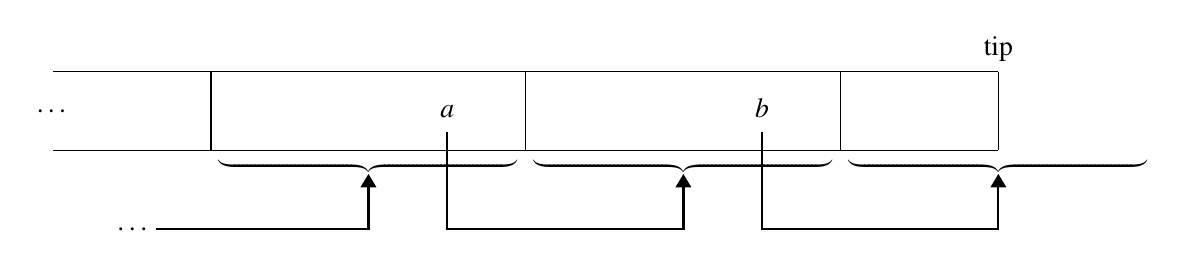
\begin{tikzpicture}
%                             /--------\
%                             |        |
%                             *        v  tip
% 1 -----+------------+------------+-----+
%        |       *    |            |     * current stake
% 0 -----+------------+------------+-----|
%   -10  -8           -4           0     2
%                |          ^
%                \----------/
\draw (-10, 0.5) node{\ldots};
\draw (-10,  0) --  (2, 0);
\draw (-10,  1) --  (2, 1);
\draw  (-8,  0) -- (-8, 1);
\draw  (-4,  0) -- (-4, 1);
\draw   (0,  0) --  (0, 1);
\draw   (2,  0) --  (2, 1) node[above]{tip};
\draw  (-6, -0.2) node {$\underbrace{\hspace{3.8cm}}$};
\draw  (-2, -0.2) node {$\underbrace{\hspace{3.8cm}}$};
\draw  ( 2, -0.2) node {$\underbrace{\hspace{3.8cm}}$};
\draw [thick, arrows={-Triangle}] (-9, -1) node[fill=white] {$\ldots$}-- (-6, -1) -- (-6, -0.3);
\draw [thick, arrows={-Triangle}] (-5, 0.5) node[fill=white] {$\mathstrut a$} -- (-5, -1) -- (-2, -1) -- (-2, -0.3);
\draw [thick, arrows={-Triangle}] (-1, 0.5) node[fill=white] {$\mathstrut b$} -- (-1, -1) -- (2, -1) -- (2, -0.3);
\end{tikzpicture}
\end{center}
%
This makes it possible to \emph{forecast} what the stake distribution (i.e.,
the ledger view) will be at various points. For example, if the chain looks like
%
\begin{center}
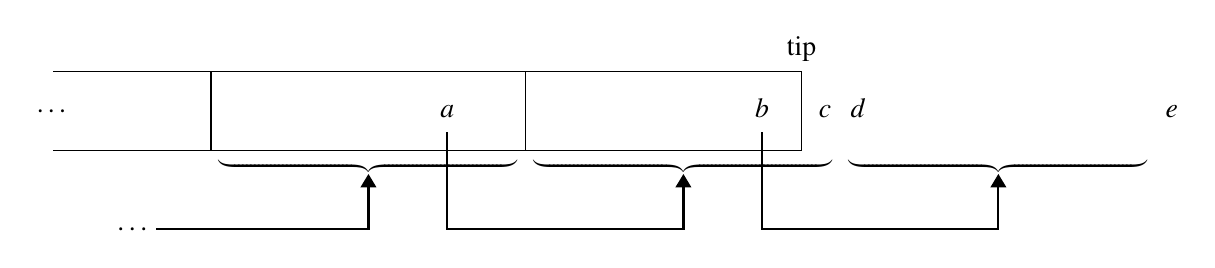
\begin{tikzpicture}
\draw (-10,    0.5) node{\ldots};
\draw (-10,    0) -- (-0.5, 0);
\draw (-10,    1) -- (-0.5, 1);
\draw  (-8,    0) -- (-8,   1);
\draw  (-4,    0) -- (-4,   1);
\draw  (-0.5,  0) -- (-0.5, 1) node[above]{tip};
\draw  (-6,   -0.2) node {$\underbrace{\hspace{3.8cm}}$};
\draw  (-2,   -0.2) node {$\underbrace{\hspace{3.8cm}}$};
\draw  ( 2,   -0.2) node {$\underbrace{\hspace{3.8cm}}$};
\draw [thick, arrows={-Triangle}] (-9, -1) node[fill=white] {$\ldots$}-- (-6, -1) -- (-6, -0.3);
\draw [thick, arrows={-Triangle}] (-5, 0.5) node[fill=white] {$\mathstrut a$} -- (-5, -1) -- (-2, -1) -- (-2, -0.3);
\draw [thick, arrows={-Triangle}] (-1, 0.5) node[fill=white] {$\mathstrut b$} -- (-1, -1) -- (2, -1) -- (2, -0.3);
\draw (0, 0.5) node[left] {$\mathstrut c$};
\draw (0, 0.5) node[right] {$\mathstrut d$};
\draw (4, 0.5) node[right] {$\mathstrut e$};
\end{tikzpicture}
\end{center}
%
then we can ``forecast'' that the stake distribution at point $c$ will be the one
established at point $a$, whereas the stake distribution at point $d$ will be the
one established at point $b$. The stake distribution at point $e$ is however not
yet known; we say that $e$ is ``out of the forecast range''.

\subsection{Code}

Since we're always forecasting what the ledger would look like \emph{if it would
be advanced to a particular slot}, the result of forecasting is always something
ticked:\footnote{Actually we never deal with an \emph{unticked} ledger view.}
%
\begin{lstlisting}
data Forecast a = Forecast {
      forecastAt  :: WithOrigin SlotNo
    , forecastFor :: SlotNo -> Except OutsideForecastRange (Ticked a)
    }
\end{lstlisting}
%
Here \lstinline!forecastAt! is the tip of the ledger in which the forecast was
constructed and \lstinline!forecastFor! is constructing the forecast for a
particular slot, possibly returning an error message of that slot is out of
range. This terminology---a forecast constructed \emph{at} a slot
and computed \emph{for} a slot---is used throughout both this technical report
as well as the consensus layer code base.

\subsection{Ledger view}
\label{forecast:ledgerview}

For the ledger view specifically, the \lstinline!LedgerSupportsProtocol!
class (\cref{ledger:api:LedgerSupportsProtocol}) requires a function
%
\begin{lstlisting}
ledgerViewForecastAt ::
     LedgerConfig blk
  -> LedgerState blk
  -> Forecast (LedgerView (BlockProtocol blk))
\end{lstlisting}
%
This function must satisfy two important properties:
%
\begin{description}
\item[Sufficient range]

When we validate headers from an upstream node, the most recent useable ledger
state we have is the ledger state at the intersection of our chain and the chain
of the upstream node. That intersection will be at most $k$ blocks back, because
that is our maximum rollback (\cref{param:k}). Furthermore, it is only useful to
track an upstream peer if we might want to adopt their blocks, and we only
switch to their chain if it is longer than ours (\cref{chain-selection}). This
means that in the worst case scenario, with the intersection $k$ blocks back, we
need to be able to evaluate $k + 1$ headers in order to adopt the alternative
chain. However, the range of a forecast is based on \emph{slots}, not blocks;
since not every slot may be contain a block\todo{We should discuss the block/slot
dichotomy somewhere}, the range needs to be sufficient to \emph{guarantee} to contain at
least $k + 1$ blocks\footnote{Due to a bug, this is not the case for Shelley,
where the effective maximum rollback is in fact $k - 1$; see
\cref{shelley:forecasting}).}; we will come back to this in
\cref{future:block-vs-slot}.

The network layer may have additional reasons for wanting a long forecast
range; see \cref{header-body}.

\item[Relation to ticking]
Forecasting is not the only way that we can get a ledger view for a particular
slot; alternatively, we can also \emph{tick} the ledger state, and then ask
for the ledger view at that ticked ledger state. These two ways should give us
the same answer:
%
\begin{equation}
\begin{array}{lllll}
\mathrm{whenever} &
\mathtt{forecastFor} \; (\mathtt{ledgerViewForecastAt}_\mathit{cfg} \; l) \; s & = & \mathtt{Right} & l' \\
\mathrm{then} & \mathtt{protocolLedgerView}_\mathit{cfg} \; (\mathtt{applyChainTick}_\mathit{cfg} \; s \; l) & = && l'
\end{array}
\end{equation}
%
In other words, whenever the ledger view for a particular slot is within the
forecast range, then ticking the ledger state to that slot and asking for the
ledger view at the tip should give the same answer. Unlike forecasting, however,
ticking has no maximum range. The reason is the following fundamental difference between these two concepts:
%
\begin{quote}
\textbf{(Forecast vs. ticking)} When we \emph{forecast} a ledger view, we are
predicting what that ledger view will be, \emph{no matter which blocks will  be
applied to the chain} between the current tip and the slot of the forecast. By
contrast , when we \emph{tick} a ledger, we are applying any time-related
changes to the ledger state in order to apply the \emph{next} block; in other
words, when we tick to a particular slot, \emph{there \emph{are} no blocks in
between the current tip and the slot we're ticking to}. Since there are no
intervening blocks, there is no uncertainty, and hence no limited range.
\end{quote}
\end{description}

\section{Queries}
\label{ledger:queries}

\chapter{State management}
\label{state}

ChainDepState, (ChainIndepState), LedgerState, ExtLedgerState

\section{Initialization}
\label{state:initialization}

Describe why it is important that we store a single snapshot and then replay
ledger events to construct the ledger DB.

\section{Header State}
\label{state:header}

\section{Extended ledger state}
\label{state:extended}

\section{Chain selection}
\label{state:chainselection}

\section{Abandoned approach: historical states}

\chapter{Epoch Boundary Blocks}
\label{ebbs}

Discuss that although EBBs are a Byron concern, their presence has far reaching
consequences on the consensus later. In hindsight, we should have tried harder
to not deal with them at all from the beginning; we did not anticipate quite how
bad the situation would be. We now have a plan for getting rid of them
(\cref{decontamination-plan}) but it will be a fairly long term thing and it
might not happen at all, depending on quite how much time is available for
removing tech debt.


\section{Introduction}

\section{Consequences}

\subsection{Chain selection}
\label{ebb-chain-selection}

\section{Elimination}
\label{decontamination-plan}

\chapter{Storage}
\label{storage}

\section{In memory}
\label{in-memory}

Describe what we store in memory, and why. Discuss chain fragments.

\section{The immutable-volatile split}
\label{immutable-volatile-split}

\section{Ledger database}
\label{storage:ledger}

\chapter{Mempool}
\label{mempool}

\section{Consistency}
\label{mempool:consistency}

Discuss that we insist on \emph{linear consistency}, and why.

\chapter{The Hard Fork Combinator}
\label{hfc}

\section{Adjustments}

In this section we discuss some adjustments we had to make to the existing
design of the consensus layer to make the HFC possible

\subsection{Simplifying chain selection}
\label{simplifying-chain-selection}

Chain selection used to be given the full fragment; now it only gets the tip.

This is non-trivial; we have a long comment explaining this for
\lstinline!preferAnchoredCandidate!; we should move (copy?) that discussion
here, and also discuss this comment from \lstinline!preferCandidate!:

\begin{lstlisting}
  -- NOTE: An assumption that is quite deeply ingrained in the design of the
  -- consensus layer is that if a chain can be extended, it always should (e.g.,
  -- see the chain database spec in @ChainDB.md@). This means that any chain
  -- is always preferred over the empty chain, and 'preferCandidate' does not
  -- need (indeed, cannot) be called if our current chain is empty.
\end{lstlisting}


\subsection{Removing the assumption that slot/time conversion is always possible}
\label{removing-known-slot-assumption}

\section{Ledger}

\subsection{Invalid states}
\label{hfc:ledger:invalid-states}

\todo{This came from the Byron/Shelley appendix. Need to generalize a bit or provide context.}
In a way, it is somewhat strange to have the hard fork mechanism be part of the
Byron (\cref{byron:hardfork}) or Shelley ledger (\cref{shelley:hardfork})
itself, rather than some overarching ledger on top. For Byron, a Byron ledger
state where the \emph{major} version is the (predetermined) moment of the hard
fork is basically an invalid state, used only once to translate to a Shelley
ledger. Similar, the \emph{hard fork} part of the Shelley protocol version will
never increase during Shelley's lifetime; the moment it \emph{does} increase,
that Shelley state will be translated to the (initial) state of the post-Shelley
ledger.

\section{Failed attempts}

\subsection{Forecasting}

As part of the integration of any ledger in the consensus layer (not HFC
specific), we need a projection from the ledger \emph{state} to the consensus
protocol ledger \emph{view}
(\cref{class:ConsensusProtocol:ledgerview,ledger:api:LedgerSupportsProtocol}).
As we have seen\todo{Once we write these sections, add back references here},
the HFC requires for each pair of consecutive eras a pair of \emph{state} translation
functions, as well as a \emph{projection} from the state of the old era to the
ledger view of the new era. These means that if we have $n + 1$ eras, we need
$n$ across-era projection functions, in addition to the $n + 1$ projections
functions we already have \emph{within} each era.

This might feel a bit cumbersome; perhaps a more natural approach would be to
only have within-era projection functions, but require a function to translate
the ledger view (in addition to the ledger state) for each pair of eras.
We initially tried this approach; when projecting from an era to the next,
we would first ask the old era to give us the final ledger view in that era,
and then translate this final ledger view across the eras:

\begin{center}
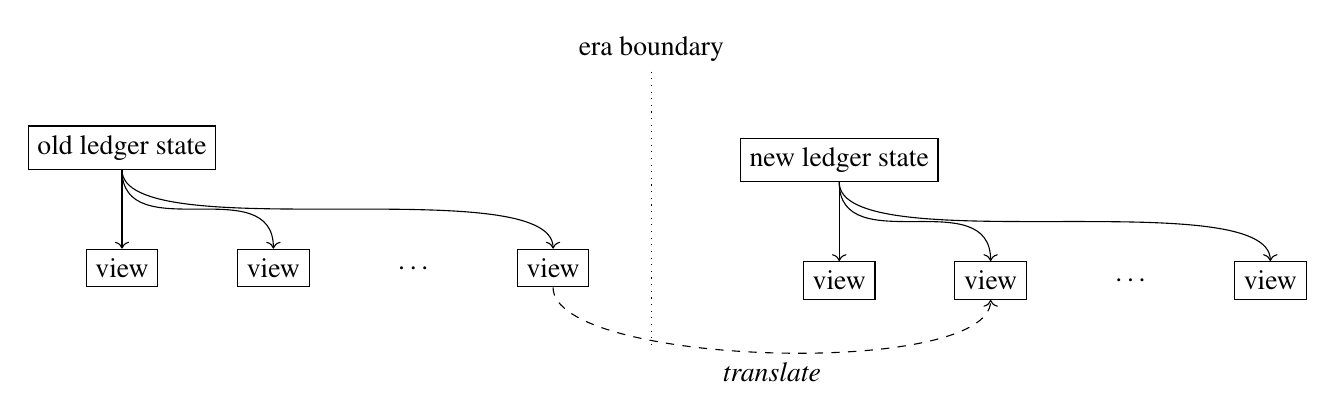
\begin{tikzpicture}[
square/.style={rectangle, draw},
]
% old ledger
\node[square] (Astate) {old ledger state};
\node[square] (Aview1) [below=of Astate] {view};
\node[square] (Aview2) [right=of Aview1] {view};
\node         (Adots)  [right=of Aview2] {$\ldots$};
\node[square] (AviewN) [right=of Adots]  {view};
\draw[->] (Astate.south) -- (Aview1.north);
\draw[->] (Astate.south) .. controls +(down:1cm) and +(up:1cm).. (Aview2.north);
\draw[->] (Astate.south) .. controls +(down:1cm) and +(up:1cm).. (AviewN.north);
%
% some intermediate nodes for positiiong
\node (AstateN) [above=of AviewN] {};
\node (mid) [right=of AstateN] {};
\node (midH) [above=of mid] {era boundary};
\node (midM) [below=of mid] {};
\node (midL) [below=of midM] {};
%
% new ledger
\node[square] (Bstate) [right=of mid] {new ledger state};
\node[square] (Bview1) [below=of Bstate] {view};
\node[square] (Bview2) [right=of Bview1] {view};
\node         (Bdots)  [right=of Bview2] {$\ldots$};
\node[square] (BviewN) [right=of Bdots]  {view};
\draw[->] (Bstate.south) -- (Bview1.north);
\draw[->] (Bstate.south) .. controls +(down:1cm) and +(up:1cm).. (Bview2.north);
\draw[->] (Bstate.south) .. controls +(down:1cm) and +(up:1cm).. (BviewN.north);
%
\draw[dotted] (midH) -- (midL);
\draw[->, dashed] (AviewN.south) .. controls +(down:1cm) and +(down:1cm) .. (Bview2.south) node[pos=0.5, below] {\emph{translate}};;
\end{tikzpicture}
\end{center}

The problem with this approach is that the ledger view only contains a small
subset of the ledger state; the old ledger \emph{state} might contain
information about scheduled changes that should be taken into account when
constructing the ledger view in the new era, but the final ledger view in the
old era might not have that information.

Indeed, a moment's reflection reveals that this cannot be right the approach.
After all, we cannot step the ledger state; the dashed arrow in
%
\begin{center}
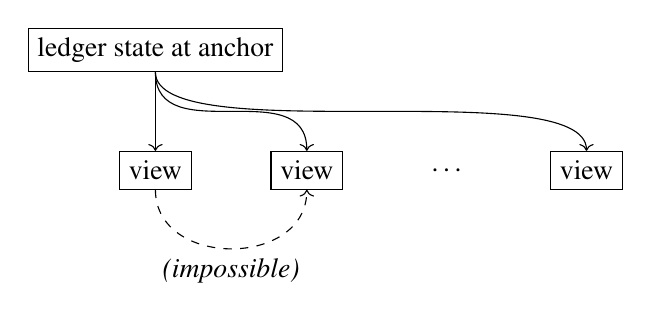
\begin{tikzpicture}[
square/.style={rectangle, draw},
]
\node[square] (state) {ledger state at anchor};
\node[square] (view1) [below=of state] {view};
\node[square] (view2) [right=of view1] {view};
\node         (dots)  [right=of view2] {$\ldots$};
\node[square] (viewN) [right=of dots]  {view};
\draw[->] (state.south) -- (view1.north);
\draw[->] (state.south) .. controls +(down:1cm) and +(up:1cm).. (view2.north);
\draw[->] (state.south) .. controls +(down:1cm) and +(up:1cm).. (viewN.north);
\draw[->, dashed] (view1.south) .. controls +(down:1cm) and +(down:1cm) .. (view2.south) node[pos=0.5, below] {\emph{(impossible)}};
\end{tikzpicture}
\end{center}
%
is not definable: scheduled changes are recorded in the ledger state, not in
the ledger view.

We cannot forecastly directly from the old ledger state to the new era either: this would result in a ledger view from the old era in the new era, violating the invariant we discussed in \cref{hfc:ledger:invalid-states}, and it would moreover result in incorrect forecast
bound checks.

Requiring a special forecasting function for each pair of eras of course in a
way is cheating: it pushes the complexity of doing this forecasting to the
specific ledgers that the HFC is instantiated at. However, as it turns out, this
function tends to be easy to define for any pair of concrete ledgers; it's just
hard to define in a completely general way.

\chapter{Testing}
\label{testing}

\section{Storage}

\section{Consensus: The New Tests}

TODO: it might be that this becomes the whole chapter, and we merely
ignore the old version.

\subsection{Dire-but-not-to-dire}
\label{testing:dire}

We should mention the PBFT threshold here \cref{bft-paper}.

\chapter{Technical design decisions}

In this chapter we will discuss a number of interesting technical decision
decisions that aren't directly to any of the specific needs of the consensus
layer.

\section{Classes versus records}
\label{classes-vs-records}

Discuss why classes are helpful (explicit about closures).

\chapter{Future work}

\section{On abstraction}

ledger integration: as things were changing a lot, it made sense for consensus to define the ledger API internally and have the integration be done consensus side. but as things are stabilizing, it might make more sense for that abstraction to live externally, so that you can literally plug in shelley into consensus and we don't have to do anything

\section{Genesis}
\label{future:genesis}

\section{On-disk ledger state}

\duncan

Sketch out what we think it could look like
Consequences for the design

\section{Transaction TTL}
\label{future:ttl}

Describe that the mempool could have explicit support for TTL, but that right now we don't (and why this is ok: the ledger anyway checks tx TTL). We should discuss why this is not an attack vector (transactions will either be included in the blockchain or else will be chucked out because some of their inputs will have been used).

\section{Block based versus slot based}
\label{future:block-vs-slot}

\section{Configuration}

What a mess.

\chapter{Conclusions}


\appendix

\chapter{Byron}

Some details specific to the Byron ledger.
EBBs already discussed at length in \cref{ebbs}.

The Byron specification can be found at \url{https://github.com/input-output-hk/cardano-ledger-specs}.

\section{Update proposals}
\label{byron:hardfork}

\subsection{Moment of hard fork}
\label{byron:hardfork:moment}

The Byron ledger state provides the current protocol version in
%
\begin{lstlisting}
adoptedProtocolVersion :: ProtocolVersion
\end{lstlisting}
%
in the \lstinline!State! type from
\lstinline!Cardano.Chain.Update.Validation.Interface!.
This protocol version is a three-tuple \emph{major}, \emph{minor}, \emph{alt}.
The Byron specification does not provide any semantic interpretation of these
components. By convention (outside of the purview of the Byron specification),
the hard fork is initiated the moment that the \emph{major} component of
\lstinline!adoptedProtocolVersion! reaches a predefined, hardcoded, value.

\subsection{The update mechanism for the \lstinline!ProtocolVersion!}

Updates to the \lstinline!ProtocolVersion! in Byron are part of the general
infrastructure for changing protocol parameters (parameters such as the maximum
block size), except that in the case of a hard fork, we care only about changing
the \lstinline!ProtocolVersion!, and not any of the parameters themselves.

The general mechanism for updating protocol parameters in Byron is as follows:

\begin{enumerate}

\item
A protocol update \emph{proposal} transaction is created. It proposes new values
for some protocol parameters and a greater \emph{protocol version} number as an
identifier. There cannot be two proposals with the same version number.

\item
Genesis key delegates can add \emph{vote} transactions that refer to such a
proposal (by its hash). They don't have to wait; a node could add a proposal and
a vote for it to its mempool simultaneously. There are only positive votes, and
a proposal has a time-to-live (see \lstinline!ppUpdateProposalTTL!) during which
to gather sufficient votes. While gathering votes, a proposal is called
\emph{active}.

Note that neither Byron nor Shelley support full centralization (everybody can
vote); this is what the Voltaire ledger is intended to accomplish.

\item
Once the number of voters satisfies a threshold (currently determined by the
\lstinline!srMinThd! field of the \lstinline!ppSoftforkRule! protocol
parameter), the proposal becomes \emph{confirmed}.

\item
Once the threshold-satisfying vote becomes stable (ie its containing block is at
least $2k$ slots deep), a block whose header's protocol version number
(\lstinline!CC.Block.headerProtocolVersion!) is that of the proposal is
interpreted as an \emph{endorsement} of the stably-confirmed proposal by the
block's issuer (specifically by the Verification Key of its delegation
certificate). Endorsements---ie \emph{any block}, since they all contain that
header field---also trigger the system to discard proposals that were not
confirmed within their TTL.

Notably, endorsements for proposals that are not yet stably-confirmed (or do not
even exist) are not invalid but rather silently ignored. In other words, no
validation applies to the `headerProtocolVersion` field.

\item
Once the number of endorsers satisfies a threshold (same as for voting), the
confirmed proposal becomes a \emph{candidate} proposal.

\item
\emph{At the beginning of an epoch}, the candidate proposal with the greatest
protocol version number among those candidates whose threshold-satisfying
endorsement is stable (ie the block is at least $2k$ deep) is \emph{adopted}:
the new protocol parameter values have now been changed.

If there was no stable candidated proposal, then nothing happens. Everything is
retained; in particular, a candidate proposal whose threshold-satisfying
endorsement was not yet stable will be adopted at the subsequent epoch unless it
is surpassed in the meantime.

When a candidate is adopted, all record of other
proposals/votes/endorsements---regardless of their state---is discarded. The
explanation for this is that such proposals would now be interpreted as an
update to the newly adopted parameter values, whereas they were validated as an
update to the previously adopted parameter values.

\end{enumerate}

The diagram shown in \cref{byron:update-process} summarizes the progress of a
proposal that's eventually adopted. For other proposals, the path short circuits
to a ``rejected/discarded'' status at some point.

\begin{figure}
\hrule
\begin{center}
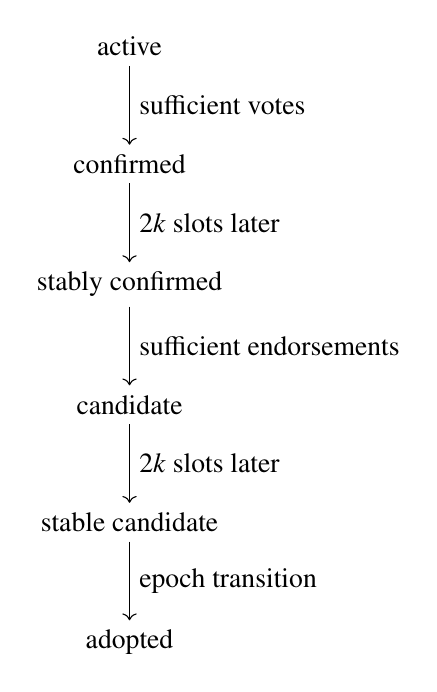
\begin{tikzpicture}
\node (act)                {active}           ;
\node (con) [below=of act] {confirmed}        ;
\node (sta) [below=of con] {stably confirmed} ;
\node (can) [below=of sta] {candidate}        ;
\node (sca) [below=of can] {stable candidate} ;
\node (ado) [below=of sca] {adopted}          ;
\draw[->] (act.south) -- (con.north) node[pos=0.5, right] {sufficient votes};
\draw[->] (con.south) -- (sta.north) node[pos=0.5, right] {$2k$ slots later};
\draw[->] (sta.south) -- (can.north) node[pos=0.5, right] {sufficient endorsements};
\draw[->] (can.south) -- (sca.north) node[pos=0.5, right] {$2k$ slots later};
\draw[->] (sca.south) -- (ado.north) node[pos=0.5, right] {epoch transition};
\end{tikzpicture}
\end{center}
\hrule
\caption{\label{byron:update-process}Byron update proposal process}
\end{figure}

\subsection{Initiating the hard fork}
\label{byron:hardfork:initiating}

Proposals to initiate the hard fork can be submitted and voted on before all
core nodes are ready. After all, once a proposal is stably confirmed, it will
effectively remain so indefinitely until nodes endorse it (or it gets superseded
by another proposal). This means that nodes can vote to initiate the hard fork,
\emph{then} wait for everybody to update their software, and once updated, the
proposal is endorsed and eventually the hard fork is initiated.

Endorsement is somewhat implicit. The node operator does not submit an explicit
``endorsement transaction'', but instead restarts the
node\footnote{\label{byron:unnecessary-restarts}A node restart is necessary for
\emph{any} change to a protocol parameter, even though most parameters do not
require any change to the software at all.} (probably after a software update
that makes the node ready to support the hard fork) with a new protocol version
(as part of a config file or command line parameter), which then gets included
in the blocks that the node produces (this value is the
\lstinline!byronProtocolVersion! field in the static \lstinline!ByronConfig!).

\subsection{Software versions}

The Byron ledger additionally also records the latest version of the software on
the chain, in order to facilitate software discovering new versions and
subsequently updating themselves. This would normally precede all of the above,
but as far as the consensus layer is concerned, this is entirely orthogonal. It
does not in any way interact with either the decision to hard fork nor the
moment of the hard fork. If we did forego it, the discussion above would still
be entirely correct. As of Shelley, software discovery is done off-chain.

The Byron \emph{block header} also records a software version
(\lstinline!headerSoftwareVersion!). This is a legacy concern only, and is
present in but ignored by the current Byron implementation, and entirely absent
from the Byron specification.

\chapter{Shelley}

\section{Update proposals}
\label{shelley:hardfork}

\subsection{Moment of the hard fork}
\label{shelley:hardfork:moment}

Similar to the Byron ledger (\cref{byron:hardfork:moment}), the Shelley ledger
provides a ``current protocol version'', but it is a two-tuple (not a
three-tuple), containing only a \emph{hard fork} component and \emph{soft fork}
component:
%
\begin{lstlisting}
_protocolVersion :: (Natural, Natural)
\end{lstlisting}
%
in \lstinline!PParams!. The hard fork from Shelley to its successor will be
initiated once the hard fork component of this version gets incremented.

\subsection{The update mechanism for the protocol version}

The update mechanism in Shelley is simpler than it is in Byron. There is no
distinction between votes and proposals: to ``vote'' for a proposal one merely
submits the exact same proposal. There is also no separate endorsement step
(though see \cref{shelley:hardfork:initiating}).

The procedure is as follows:

\begin{enumerate}

\item
As in Byron, a proposal is a partial map from parameters to their values.

\item
During each epoch, a genesis key can submit (via its delegates) zero, one, or
many proposals; each submission overrides the previous one.

\item
``Voting'' (submitting of proposals) ends $6k/f$ slots before the end of the
epoch (i.e., twice the stability period, called \lstinline!stabilityWindow! in
the Shelley ledger implementation).

\item
At the end of an epoch, if the majority of nodes (as determined by the
\lstinline!Quorum! specification constant, which must be greater than half the
nodes) have most recently submitted the same exact proposal, then it is adopted.

\item
The next epoch is always started with a clean slate, proposals from the
previous epoch that didn't make it are discarded.\footnote{Proposals \emph{can}
be explicitly marked to be for future epochs; in that case, these are simply
not considered until that epoch is reached.}

\end{enumerate}

The protocol version itself is also considered to be merely another parameter,
and parameters can change without changing the protocol version, although a
convention could be established that the protocol version must change if any of
the parameters do; but the specification itself does not mandate this.

\subsection{Initiating the hard fork}
\label{shelley:hardfork:initiating}

The timing of the hard fork in Shelley is different to the one in Byron: in
Byron, we \emph{first} vote and then wait for people to get ready
(\cref{byron:hardfork:initiating}); in Shelley it is the other way around.

Core node operators will want to know that a significant majority of the core
nodes is ready (supports the hard fork) before initiating it. To make this
visible, Shelley blocks contain a protocol version. This is not related to the
current protocol version as reported by the ledger state
(\lstinline!_protocolVersion! as discussed in the previous section), but it is
the \emph{maximum} protocol version that the node which produced that block can
support.

Once we see blocks from all or nearly all core nodes with the `hard fork`
component of their protocol version equal to the post-hard-fork value, nodes
will submit their proposals with the required major version change to initiate
the hard fork.\footnote{This also means that unlike in Byron
(\cref{byron:unnecessary-restarts}), in Shelley there is no need to restart the
node merely to support a particular parameter change (such as a maximum block
size).}

\section{Forecasting}
\label{shelley:forecasting}

Discuss the fact that the effective maximum rollback in Shelley is $k - 1$,
not $k$; see also \cref{ledger:forecasting}.


\bibliographystyle{acm}
\bibliography{references}

\end{document}
